% Figure from MATH 591 notes, section 70. Added (Lecture 25): flow boxes covering a compact manifold (user's figure).
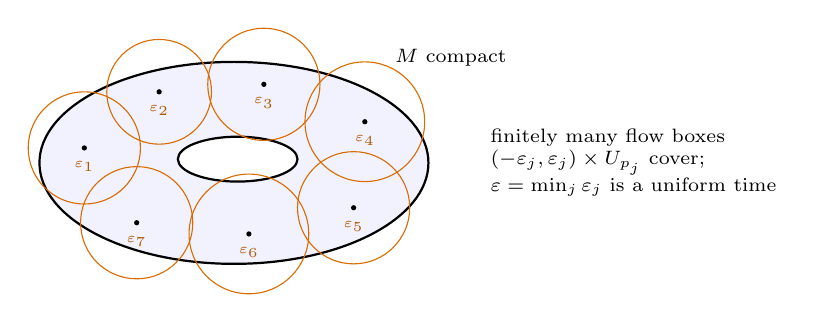
\begin{tikzpicture}[scale=0.95]
\draw[thick, fill=blue!5] (0,0) ellipse (2.6 and 1.35);
\fill[white] (0.05,0.05) ellipse (0.8 and 0.3); \draw[thick] (0.05,0.05) ellipse (0.8 and 0.3);
\draw[orange!85!black] (-2.0,0.2) circle (0.75); \fill (-2.0,0.2) circle (1pt); \node[font=\tiny, orange!70!black] at (-2.0,-0.05) {$\varepsilon_{1}$};
\draw[orange!85!black] (-1.0,0.95) circle (0.7); \fill (-1.0,0.95) circle (1pt); \node[font=\tiny, orange!70!black] at (-1.0,0.70) {$\varepsilon_{2}$};
\draw[orange!85!black] (0.4,1.05) circle (0.75); \fill (0.4,1.05) circle (1pt); \node[font=\tiny, orange!70!black] at (0.4,0.80) {$\varepsilon_{3}$};
\draw[orange!85!black] (1.75,0.55) circle (0.8); \fill (1.75,0.55) circle (1pt); \node[font=\tiny, orange!70!black] at (1.75,0.30) {$\varepsilon_{4}$};
\draw[orange!85!black] (1.6,-0.6) circle (0.75); \fill (1.6,-0.6) circle (1pt); \node[font=\tiny, orange!70!black] at (1.6,-0.85) {$\varepsilon_{5}$};
\draw[orange!85!black] (0.2,-0.95) circle (0.8); \fill (0.2,-0.95) circle (1pt); \node[font=\tiny, orange!70!black] at (0.2,-1.20) {$\varepsilon_{6}$};
\draw[orange!85!black] (-1.3,-0.8) circle (0.75); \fill (-1.3,-0.8) circle (1pt); \node[font=\tiny, orange!70!black] at (-1.3,-1.05) {$\varepsilon_{7}$};
\node[font=\scriptsize] at (2.9,1.4) {$M$ compact};
\node[font=\scriptsize, anchor=west, align=left] at (3.3,0.0) {finitely many flow boxes\\ $(-\varepsilon_j, \varepsilon_j) \times U_{p_j}$ cover;\\ $\varepsilon = \min_j \varepsilon_j$ is a uniform time};
\end{tikzpicture}
